%% LyX 2.0.3 created this file.  For more info, see http://www.lyx.org/.
%% Do not edit unless you really know what you are doing.
\documentclass[a4paper,oneside,english]{scrbook}
\renewcommand{\rmdefault}{cmr}
\renewcommand{\sfdefault}{cmss}
\renewcommand{\ttdefault}{cmtt}
\renewcommand{\familydefault}{\sfdefault}
\usepackage[T1]{fontenc}
\usepackage[latin9]{inputenc}
\usepackage{listings}
\setcounter{secnumdepth}{3}
\setcounter{tocdepth}{3}
\setlength{\parskip}{\medskipamount}
\setlength{\parindent}{0pt}
\usepackage{color}
\usepackage{babel}
\usepackage{float}
\usepackage{textcomp}
\usepackage{graphicx}
\usepackage{setspace}
\onehalfspacing
\usepackage[unicode=true,
 bookmarks=true,bookmarksnumbered=true,bookmarksopen=true,bookmarksopenlevel=1,
 breaklinks=true,pdfborder={0 0 0},backref=false,colorlinks=true]
 {hyperref}
\hypersetup{pdftitle={GPS Evaluator},
 pdfauthor={T. Himmer, M. Wydler, K-H. Zimmermann}}

\makeatletter

%%%%%%%%%%%%%%%%%%%%%%%%%%%%%% LyX specific LaTeX commands.
\pdfpageheight\paperheight
\pdfpagewidth\paperwidth


%%%%%%%%%%%%%%%%%%%%%%%%%%%%%% Textclass specific LaTeX commands.
\newcommand{\lyxaddress}[1]{
\par {\raggedright #1
\vspace{1.4em}
\noindent\par}
}

%%%%%%%%%%%%%%%%%%%%%%%%%%%%%% User specified LaTeX commands.
\usepackage{fancyvrb}
\usepackage{color}
\usepackage{fancyhdr}
\setlength{\headheight}{15pt}

\pagestyle{fancy}
\renewcommand{\chaptermark}[1]{ \markboth{#1}{} }
\renewcommand{\sectionmark}[1]{ \markright{#1}{} }

\fancyhf{}
\fancyhead[LE,RO]{\thepage}
\fancyhead[RE]{\textit{ \nouppercase{\leftmark}} }
\fancyhead[LO]{\textit{ \nouppercase{\rightmark}} }

\fancypagestyle{plain}{ %
  \fancyhf{} % remove everything
  \renewcommand{\headrulewidth}{0pt} % remove lines as well
  \renewcommand{\footrulewidth}{0pt}
}


\makeatletter
\def\PY@reset{\let\PY@it=\relax \let\PY@bf=\relax%
    \let\PY@ul=\relax \let\PY@tc=\relax%
    \let\PY@bc=\relax \let\PY@ff=\relax}
\def\PY@tok#1{\csname PY@tok@#1\endcsname}
\def\PY@toks#1+{\ifx\relax#1\empty\else%
    \PY@tok{#1}\expandafter\PY@toks\fi}
\def\PY@do#1{\PY@bc{\PY@tc{\PY@ul{%
    \PY@it{\PY@bf{\PY@ff{#1}}}}}}}
\def\PY#1#2{\PY@reset\PY@toks#1+\relax+\PY@do{#2}}

\expandafter\def\csname PY@tok@gd\endcsname{\def\PY@tc##1{\textcolor[rgb]{0.63,0.00,0.00}{##1}}}
\expandafter\def\csname PY@tok@gu\endcsname{\let\PY@bf=\textbf\def\PY@tc##1{\textcolor[rgb]{0.50,0.00,0.50}{##1}}}
\expandafter\def\csname PY@tok@gt\endcsname{\def\PY@tc##1{\textcolor[rgb]{0.00,0.27,0.87}{##1}}}
\expandafter\def\csname PY@tok@gs\endcsname{\let\PY@bf=\textbf}
\expandafter\def\csname PY@tok@gr\endcsname{\def\PY@tc##1{\textcolor[rgb]{1.00,0.00,0.00}{##1}}}
\expandafter\def\csname PY@tok@cm\endcsname{\def\PY@tc##1{\textcolor[rgb]{0.53,0.53,0.53}{##1}}}
\expandafter\def\csname PY@tok@vg\endcsname{\let\PY@bf=\textbf\def\PY@tc##1{\textcolor[rgb]{0.87,0.47,0.00}{##1}}}
\expandafter\def\csname PY@tok@m\endcsname{\let\PY@bf=\textbf\def\PY@tc##1{\textcolor[rgb]{0.40,0.00,0.93}{##1}}}
\expandafter\def\csname PY@tok@mh\endcsname{\let\PY@bf=\textbf\def\PY@tc##1{\textcolor[rgb]{0.00,0.33,0.53}{##1}}}
\expandafter\def\csname PY@tok@cs\endcsname{\let\PY@bf=\textbf\def\PY@tc##1{\textcolor[rgb]{0.80,0.00,0.00}{##1}}}
\expandafter\def\csname PY@tok@ge\endcsname{\let\PY@it=\textit}
\expandafter\def\csname PY@tok@vc\endcsname{\def\PY@tc##1{\textcolor[rgb]{0.20,0.40,0.60}{##1}}}
\expandafter\def\csname PY@tok@il\endcsname{\let\PY@bf=\textbf\def\PY@tc##1{\textcolor[rgb]{0.00,0.00,0.87}{##1}}}
\expandafter\def\csname PY@tok@go\endcsname{\def\PY@tc##1{\textcolor[rgb]{0.53,0.53,0.53}{##1}}}
\expandafter\def\csname PY@tok@cp\endcsname{\def\PY@tc##1{\textcolor[rgb]{0.33,0.47,0.60}{##1}}}
\expandafter\def\csname PY@tok@gi\endcsname{\def\PY@tc##1{\textcolor[rgb]{0.00,0.63,0.00}{##1}}}
\expandafter\def\csname PY@tok@gh\endcsname{\let\PY@bf=\textbf\def\PY@tc##1{\textcolor[rgb]{0.00,0.00,0.50}{##1}}}
\expandafter\def\csname PY@tok@ni\endcsname{\let\PY@bf=\textbf\def\PY@tc##1{\textcolor[rgb]{0.53,0.00,0.00}{##1}}}
\expandafter\def\csname PY@tok@nl\endcsname{\let\PY@bf=\textbf\def\PY@tc##1{\textcolor[rgb]{0.60,0.47,0.00}{##1}}}
\expandafter\def\csname PY@tok@nn\endcsname{\let\PY@bf=\textbf\def\PY@tc##1{\textcolor[rgb]{0.05,0.52,0.71}{##1}}}
\expandafter\def\csname PY@tok@no\endcsname{\let\PY@bf=\textbf\def\PY@tc##1{\textcolor[rgb]{0.00,0.20,0.40}{##1}}}
\expandafter\def\csname PY@tok@na\endcsname{\def\PY@tc##1{\textcolor[rgb]{0.00,0.00,0.80}{##1}}}
\expandafter\def\csname PY@tok@nb\endcsname{\def\PY@tc##1{\textcolor[rgb]{0.00,0.44,0.13}{##1}}}
\expandafter\def\csname PY@tok@nc\endcsname{\let\PY@bf=\textbf\def\PY@tc##1{\textcolor[rgb]{0.73,0.00,0.40}{##1}}}
\expandafter\def\csname PY@tok@nd\endcsname{\let\PY@bf=\textbf\def\PY@tc##1{\textcolor[rgb]{0.33,0.33,0.33}{##1}}}
\expandafter\def\csname PY@tok@ne\endcsname{\let\PY@bf=\textbf\def\PY@tc##1{\textcolor[rgb]{1.00,0.00,0.00}{##1}}}
\expandafter\def\csname PY@tok@nf\endcsname{\let\PY@bf=\textbf\def\PY@tc##1{\textcolor[rgb]{0.00,0.40,0.73}{##1}}}
\expandafter\def\csname PY@tok@si\endcsname{\def\PY@bc##1{\setlength{\fboxsep}{0pt}\colorbox[rgb]{0.93,0.93,0.93}{\strut ##1}}}
\expandafter\def\csname PY@tok@s2\endcsname{\def\PY@bc##1{\setlength{\fboxsep}{0pt}\colorbox[rgb]{1.00,0.94,0.94}{\strut ##1}}}
\expandafter\def\csname PY@tok@vi\endcsname{\def\PY@tc##1{\textcolor[rgb]{0.20,0.20,0.73}{##1}}}
\expandafter\def\csname PY@tok@nt\endcsname{\def\PY@tc##1{\textcolor[rgb]{0.00,0.47,0.00}{##1}}}
\expandafter\def\csname PY@tok@nv\endcsname{\def\PY@tc##1{\textcolor[rgb]{0.60,0.40,0.20}{##1}}}
\expandafter\def\csname PY@tok@s1\endcsname{\def\PY@bc##1{\setlength{\fboxsep}{0pt}\colorbox[rgb]{1.00,0.94,0.94}{\strut ##1}}}
\expandafter\def\csname PY@tok@gp\endcsname{\let\PY@bf=\textbf\def\PY@tc##1{\textcolor[rgb]{0.78,0.36,0.04}{##1}}}
\expandafter\def\csname PY@tok@sh\endcsname{\def\PY@bc##1{\setlength{\fboxsep}{0pt}\colorbox[rgb]{1.00,0.94,0.94}{\strut ##1}}}
\expandafter\def\csname PY@tok@ow\endcsname{\let\PY@bf=\textbf\def\PY@tc##1{\textcolor[rgb]{0.00,0.00,0.00}{##1}}}
\expandafter\def\csname PY@tok@sx\endcsname{\def\PY@tc##1{\textcolor[rgb]{0.87,0.13,0.00}{##1}}\def\PY@bc##1{\setlength{\fboxsep}{0pt}\colorbox[rgb]{1.00,0.94,0.94}{\strut ##1}}}
\expandafter\def\csname PY@tok@bp\endcsname{\def\PY@tc##1{\textcolor[rgb]{0.00,0.44,0.13}{##1}}}
\expandafter\def\csname PY@tok@c1\endcsname{\def\PY@tc##1{\textcolor[rgb]{0.53,0.53,0.53}{##1}}}
\expandafter\def\csname PY@tok@kc\endcsname{\let\PY@bf=\textbf\def\PY@tc##1{\textcolor[rgb]{0.00,0.53,0.00}{##1}}}
\expandafter\def\csname PY@tok@c\endcsname{\def\PY@tc##1{\textcolor[rgb]{0.53,0.53,0.53}{##1}}}
\expandafter\def\csname PY@tok@mf\endcsname{\let\PY@bf=\textbf\def\PY@tc##1{\textcolor[rgb]{0.40,0.00,0.93}{##1}}}
\expandafter\def\csname PY@tok@err\endcsname{\def\PY@tc##1{\textcolor[rgb]{1.00,0.00,0.00}{##1}}\def\PY@bc##1{\setlength{\fboxsep}{0pt}\colorbox[rgb]{1.00,0.67,0.67}{\strut ##1}}}
\expandafter\def\csname PY@tok@kd\endcsname{\let\PY@bf=\textbf\def\PY@tc##1{\textcolor[rgb]{0.00,0.53,0.00}{##1}}}
\expandafter\def\csname PY@tok@ss\endcsname{\def\PY@tc##1{\textcolor[rgb]{0.67,0.40,0.00}{##1}}}
\expandafter\def\csname PY@tok@sr\endcsname{\def\PY@tc##1{\textcolor[rgb]{0.00,0.00,0.00}{##1}}\def\PY@bc##1{\setlength{\fboxsep}{0pt}\colorbox[rgb]{1.00,0.94,1.00}{\strut ##1}}}
\expandafter\def\csname PY@tok@mo\endcsname{\let\PY@bf=\textbf\def\PY@tc##1{\textcolor[rgb]{0.27,0.00,0.93}{##1}}}
\expandafter\def\csname PY@tok@mi\endcsname{\let\PY@bf=\textbf\def\PY@tc##1{\textcolor[rgb]{0.00,0.00,0.87}{##1}}}
\expandafter\def\csname PY@tok@kn\endcsname{\let\PY@bf=\textbf\def\PY@tc##1{\textcolor[rgb]{0.00,0.53,0.00}{##1}}}
\expandafter\def\csname PY@tok@o\endcsname{\def\PY@tc##1{\textcolor[rgb]{0.20,0.20,0.20}{##1}}}
\expandafter\def\csname PY@tok@kr\endcsname{\let\PY@bf=\textbf\def\PY@tc##1{\textcolor[rgb]{0.00,0.53,0.00}{##1}}}
\expandafter\def\csname PY@tok@s\endcsname{\def\PY@bc##1{\setlength{\fboxsep}{0pt}\colorbox[rgb]{1.00,0.94,0.94}{\strut ##1}}}
\expandafter\def\csname PY@tok@kp\endcsname{\let\PY@bf=\textbf\def\PY@tc##1{\textcolor[rgb]{0.00,0.20,0.53}{##1}}}
\expandafter\def\csname PY@tok@w\endcsname{\def\PY@tc##1{\textcolor[rgb]{0.73,0.73,0.73}{##1}}}
\expandafter\def\csname PY@tok@kt\endcsname{\let\PY@bf=\textbf\def\PY@tc##1{\textcolor[rgb]{0.20,0.20,0.60}{##1}}}
\expandafter\def\csname PY@tok@sc\endcsname{\def\PY@tc##1{\textcolor[rgb]{0.00,0.27,0.87}{##1}}}
\expandafter\def\csname PY@tok@sb\endcsname{\def\PY@bc##1{\setlength{\fboxsep}{0pt}\colorbox[rgb]{1.00,0.94,0.94}{\strut ##1}}}
\expandafter\def\csname PY@tok@k\endcsname{\let\PY@bf=\textbf\def\PY@tc##1{\textcolor[rgb]{0.00,0.53,0.00}{##1}}}
\expandafter\def\csname PY@tok@se\endcsname{\let\PY@bf=\textbf\def\PY@tc##1{\textcolor[rgb]{0.40,0.40,0.40}{##1}}\def\PY@bc##1{\setlength{\fboxsep}{0pt}\colorbox[rgb]{1.00,0.94,0.94}{\strut ##1}}}
\expandafter\def\csname PY@tok@sd\endcsname{\def\PY@tc##1{\textcolor[rgb]{0.87,0.27,0.13}{##1}}}

\def\PYZbs{\char`\\}
\def\PYZus{\char`\_}
\def\PYZob{\char`\{}
\def\PYZcb{\char`\}}
\def\PYZca{\char`\^}
\def\PYZam{\char`\&}
\def\PYZlt{\char`\<}
\def\PYZgt{\char`\>}
\def\PYZsh{\char`\#}
\def\PYZpc{\char`\%}
\def\PYZdl{\char`\$}
\def\PYZhy{\char`\-}
\def\PYZsq{\char`\'}
\def\PYZdq{\char`\"}
\def\PYZti{\char`\~}
% for compatibility with earlier versions
\def\PYZat{@}
\def\PYZlb{[}
\def\PYZrb{]}
\makeatother

\makeatother

\begin{document}

\subject{Mixed Signal, Hard-Software-Co-Design\\
(Embedded Systems)}


\title{{\Huge GPS Evaluator}}


\subtitle{{\Large Charaterization of oscialltors}}


\author{Tobias Himmer\\
Michael Wydler\\
Karl-Heinz Zimmermann}


\date{19.01.2013}


\publishers{
\includegraphics[width=0.4\textwidth]{images/HS_RV_Logo_english}}

\maketitle
\cleardoublepage{}

\tableofcontents{}

\pagebreak{}


\chapter{Basics}

The GPS Evaluator shall display the system's position as reported
by the GPS module (the position is retrieved using at least 3 satellites).
The system (Figure \ref{fig:Overview-of-the-system}) uses the GPS
clock as reference signal for further time measurements on the Spartan
3E board. The clock deviation of both, the internal system clock and
the external oscillator is calculated. The calculated values and the
GPS position are sent to a server. It is also possible to connect
multiple smartphones to the server, which also send their actual position.
The position of the GPS board and the smartphones can be displayed
using any%
\footnote{Internet Explorer excluded%
} webbrowser.

\begin{figure}[h]
\noindent \begin{centering}
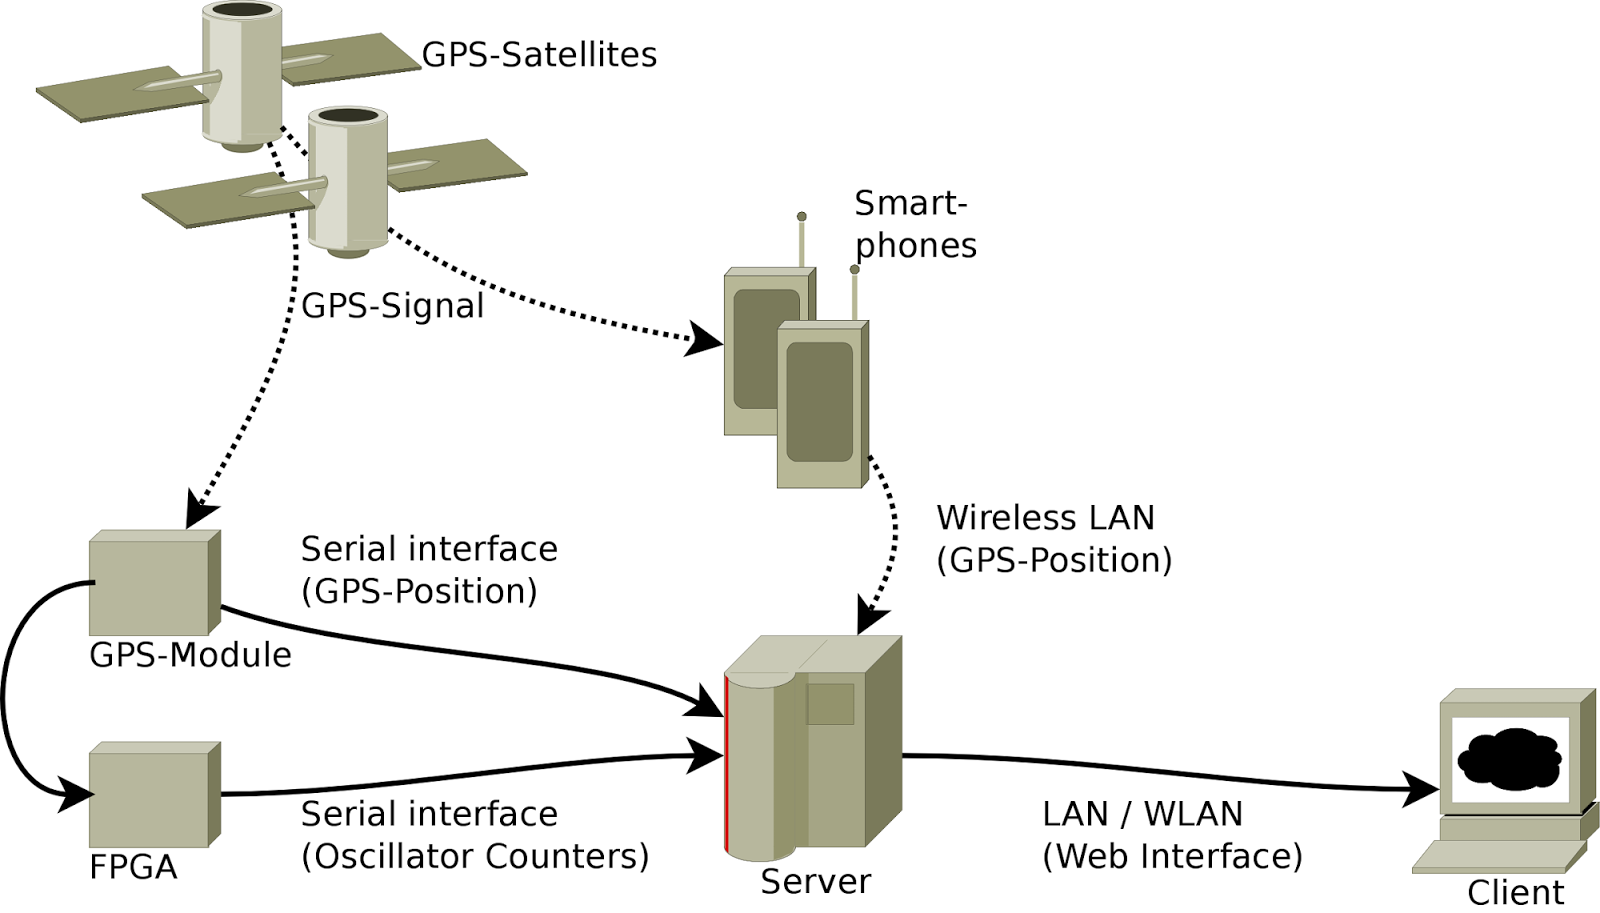
\includegraphics[width=1\textwidth]{images/system_overview}
\par\end{centering}

\caption{\label{fig:Overview-of-the-system}Overview of the complete system.}
\end{figure}



\section{Concept of GPS}

The GPS is using the time-delay of the travelling signal to determine
the current position. Therefor at least 3 satellites are required
(Figure \ref{fig:Concept-of-GPS}). The satellites need a synchronized
and very accurate clock to get an accurate position. A fourth satellite
is required to get an accurate time signal. This time signal is well
suited for characterizing an oscillator\textquoteright{}s frequency
and hence used as the reference time signal in this project.

\begin{figure}[h]
\noindent \begin{centering}
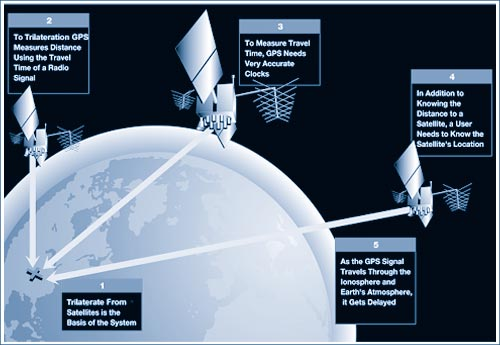
\includegraphics[width=0.75\textwidth]{images/gps_concept}
\par\end{centering}

\caption{\label{fig:Concept-of-GPS}Concept of GPS}
\end{figure}


For more information, please see \cite{GPSWorld:1990:GPS}.


\section{NMEA Protocol}

NMEA 0183 is a standardised communication protocol, which was defined
by the National Marine Electronics Association (NMEA). It is used
for the communication between GPS devices and computers. The data
sent with this protocol is structured in so-called sentences and have
the following format:

\texttt{\$SDDBT,22.3,f,6.8,M,3.7,F{*}3F<cr><lf>}

The \textquotedblleft{}\texttt{\$}\textquotedblright{} character indicates
a new sentence and the \textquotedblleft{}\texttt{{*}}\textquotedblright{}
character indicates the end. After \textquotedblleft{}\texttt{{*}}\textquotedblright{}
it follows the check-sum (XOR of all characters between the \textquotedblleft{}\texttt{\$}\textquotedblright{}
and \textquotedblleft{}\texttt{{*}}\textquotedblright{}) of the sentence.

For this implementation only 3 of over 50 possible sentences are used:
\begin{itemize}
\item \textbf{GPRMC}\\
Recommended Minimum Sentence C, supported by every GPS device. Contains
information about date, time, status and mode.
\item \textbf{GPGGA}\\
Contains the most important information about position, height and
accuracy.
\item \textbf{GPGSA}\\
Contains information about fixed satellites, fix quality and accuracy.
\end{itemize}
For detailed information about MNEA sentences refer to \cite{Glenn:2001:NMEA}
and \cite{Wiki:2012:NMEA}.


\chapter{FPGA}


\section{Overview}

\begin{figure}[h]
\noindent \begin{centering}
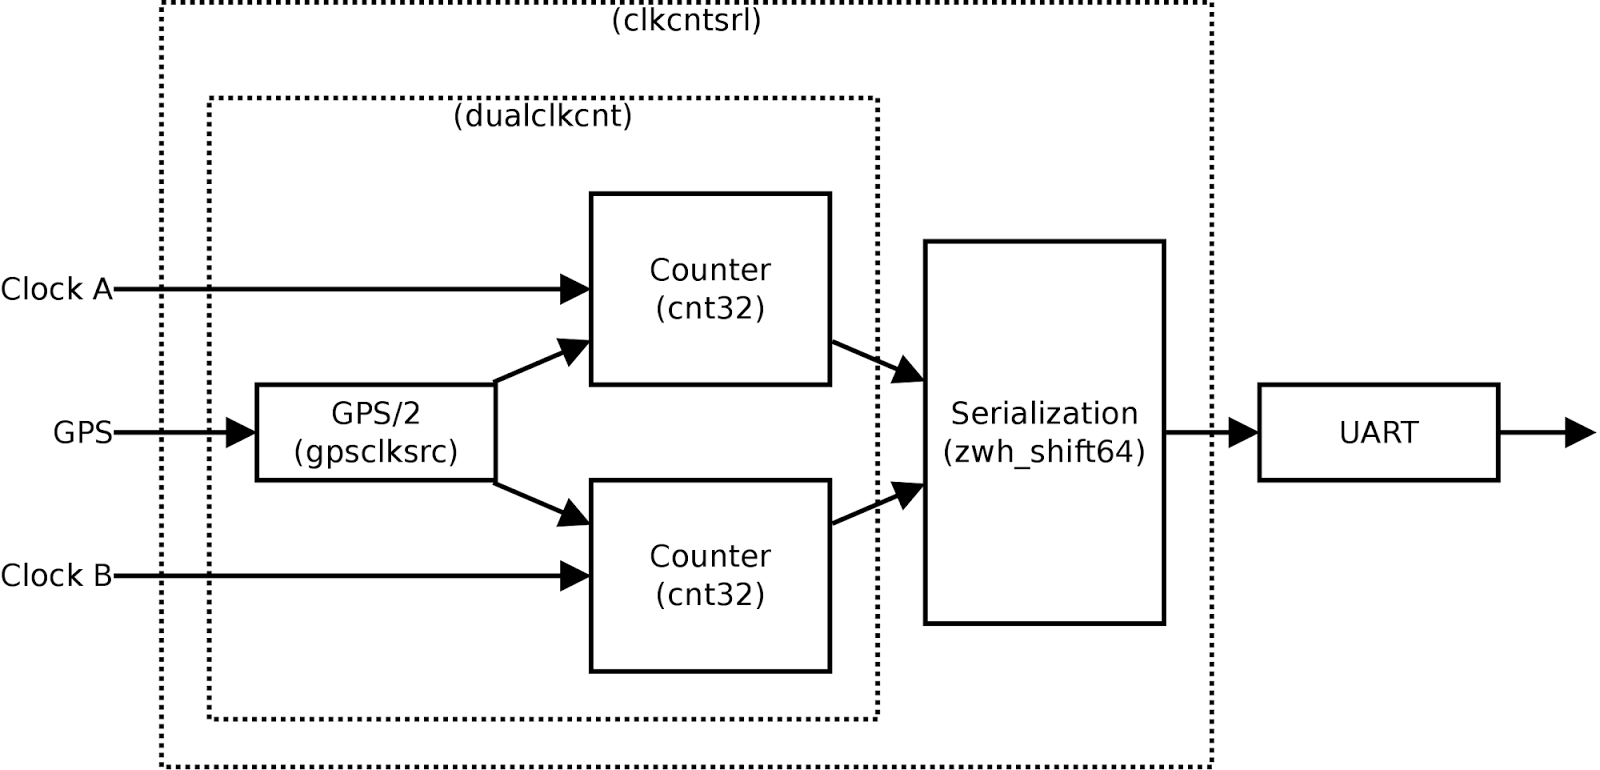
\includegraphics[width=1\textwidth]{images/fpga_overview}
\par\end{centering}

\caption{\label{fig:FPGA-Overview}Overview}
\end{figure}


Clock A is used as system clock - e.g. edge detectors use this clock
source as reference. Thus, clock A should always be faster than clock
B!

The internal circuit for the FPGA is divided in the following tasks:
\begin{itemize}
\item Generation of the halved GPS clock signal as well as detecting rising
and falling edges of the halved GPS clock signal.
\item Counting of the frequency for both oscillator inputs in parallel.
\item Serializing the counter values.
\item Sending the serialized counter values to a computer for visualization.
\end{itemize}
These tasks are divided into two phases, each one second in duration,
depending on the halved GPS clock signal:
\begin{itemize}
\item Clock signal equals logical one: Both connected frequencies are counted
until the end of phase 1, then held for further processing.
\item Clock signal equals logical zero: Serializing and sending the previously
determined counter values via UART. At the end of phase two the counters
are reset into their initial state to prepare for counting frequencies
in the next cycle.
\end{itemize}
Therefore every two seconds, a new pair of counter values is generated
and sent to the connected device. Figure \ref{fig:The-two-phases-of-the-FPGA}
illustrates one measurement and transmission cycle.

\begin{figure}[h]
\noindent \begin{centering}
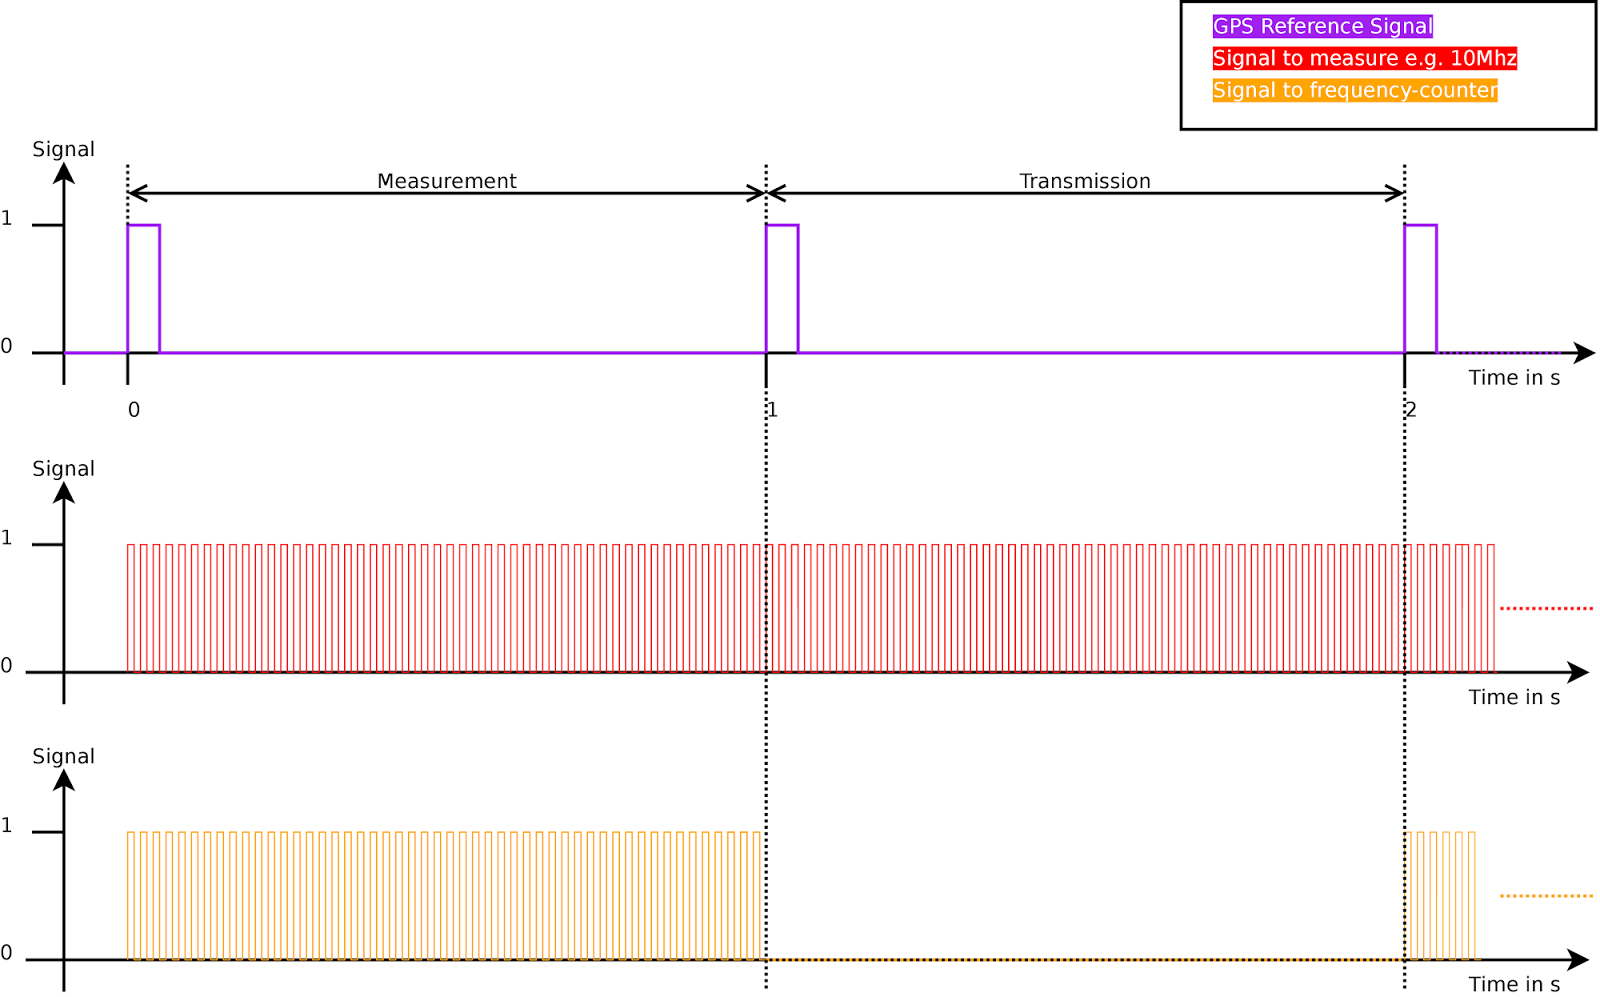
\includegraphics[width=1\textwidth]{images/fpga_phases}
\par\end{centering}

\caption{\label{fig:The-two-phases-of-the-FPGA}The two phases of the FPGA}
\end{figure}



\section{GPS Clock}

\begin{figure}[h]
\noindent \begin{centering}
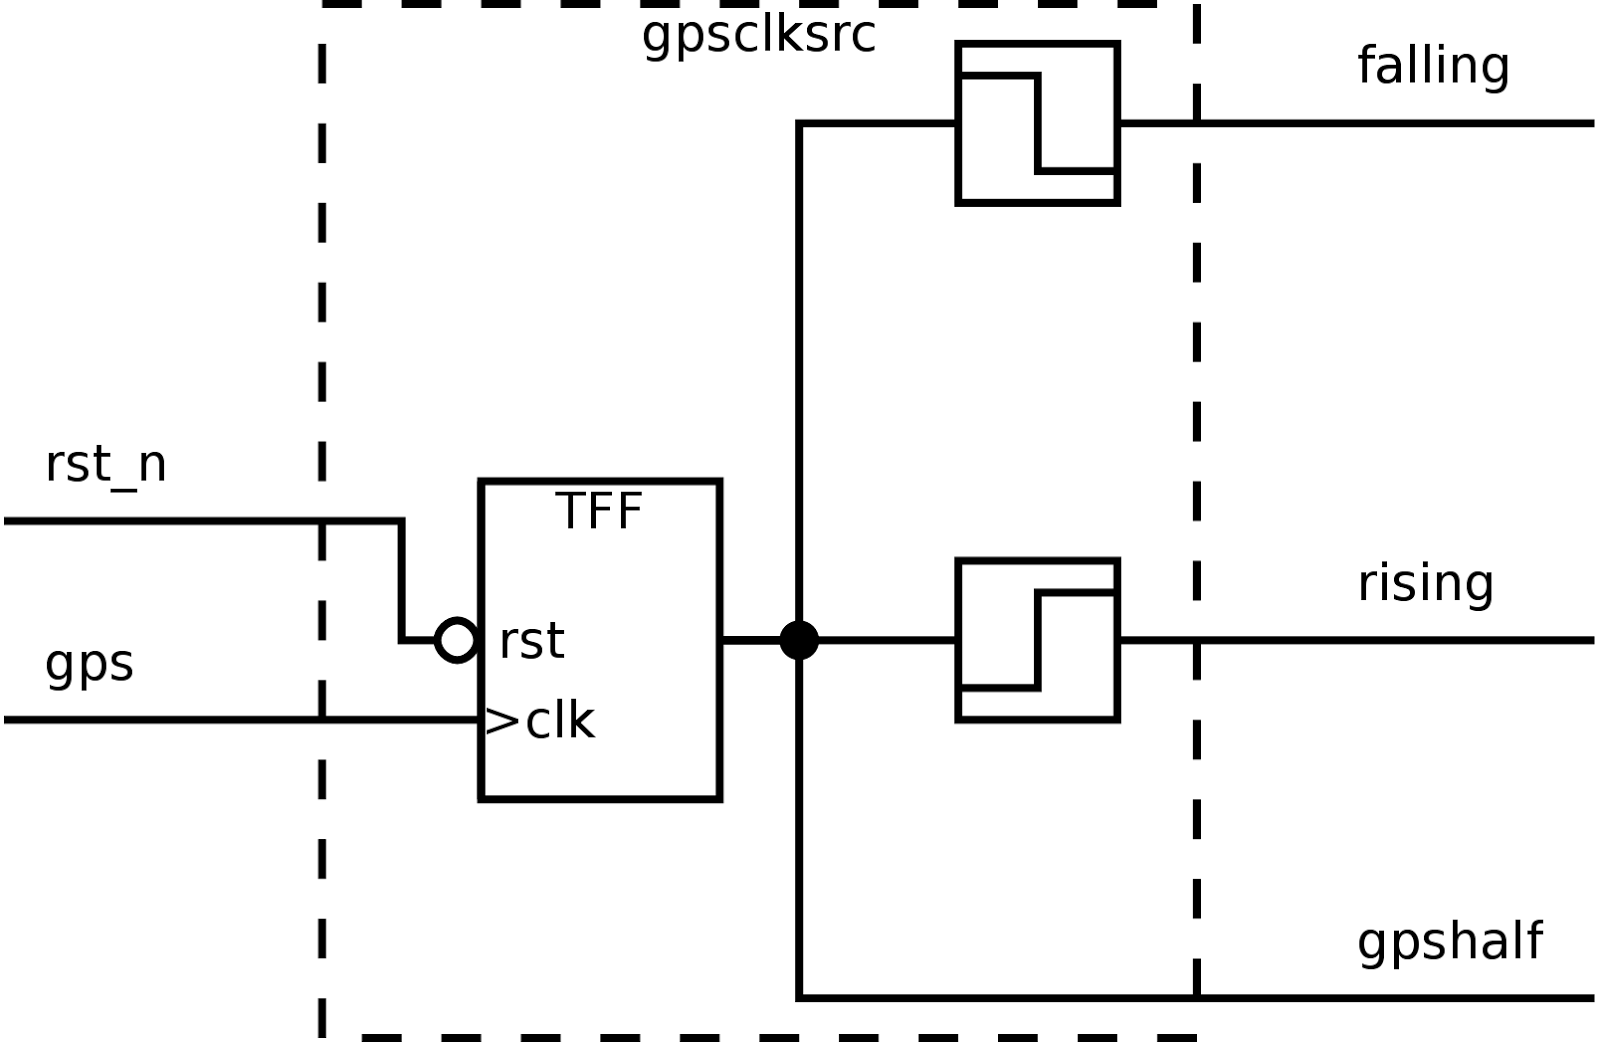
\includegraphics[width=0.5\textwidth]{images/fpga_clock_divider}
\par\end{centering}

\caption{\label{fig:GPS-clock-divider}GPS clock divider and edge detectors}
\end{figure}


The GPS clock passes a toggle flip-flop to generate the halved GPS
clock (Figure \ref{fig:GPS-clock-divider}). Additionally the falling
and rising edges are detected: A pulse on the rising edge output marks
the beginning of a measurement-phase, whereas a falling edge marks
the end of the measurement-phase and the beginning of a transmission-phase.


\section{\label{sec:2x32-Bit-Binary-Counter}2x32-Bit Binary Counter}

\begin{figure}[H]
\noindent \begin{centering}
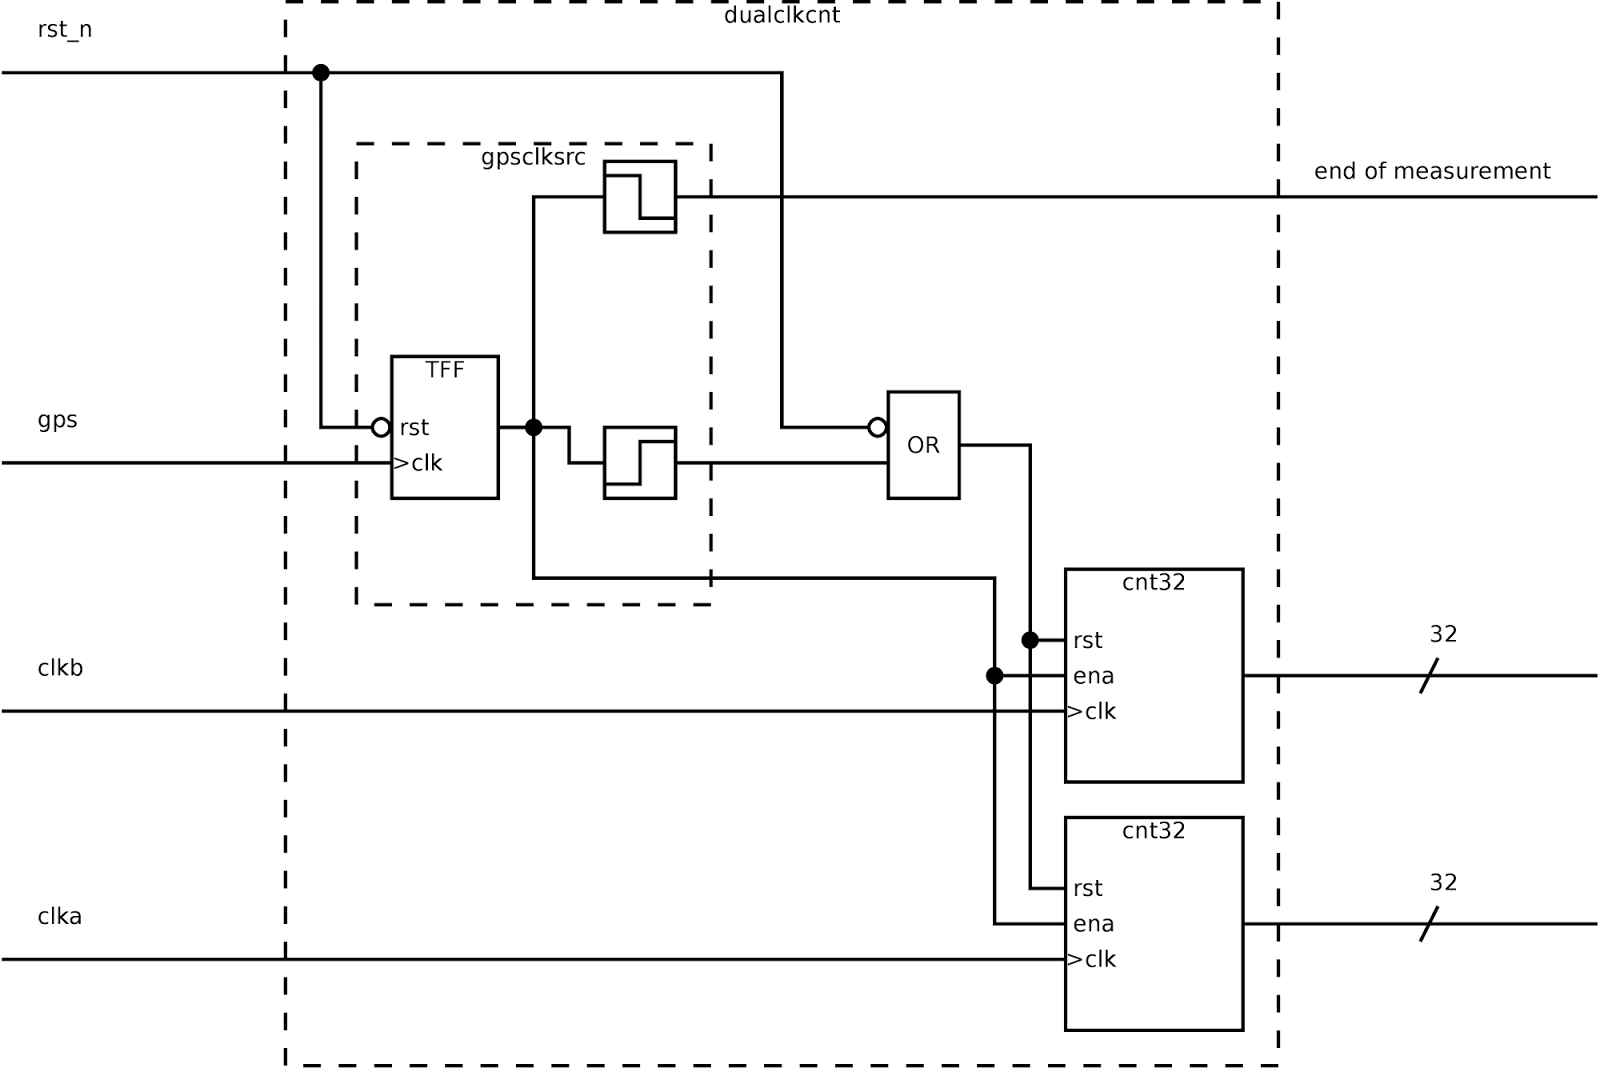
\includegraphics[width=0.85\textwidth]{images/fpga_counters}
\par\end{centering}

\caption{\label{fig:32-bit-binary-counters}32-bit binary counters}
\end{figure}


Frequency counting is implemented using a 32-bit binary counter for
each oscillator input (Figure \ref{fig:32-bit-binary-counters}).
No clock dividers for the oscillator inputs are used in this design.
Each counter ranges from 0 to 4.294.967.295 (2\textthreesuperior{}\texttwosuperior{}-1),
hence frequencies up to \textasciitilde{}4.294GHz could be counted
for one second.


\section{Serialization}

\begin{figure}[h]
\noindent \begin{centering}
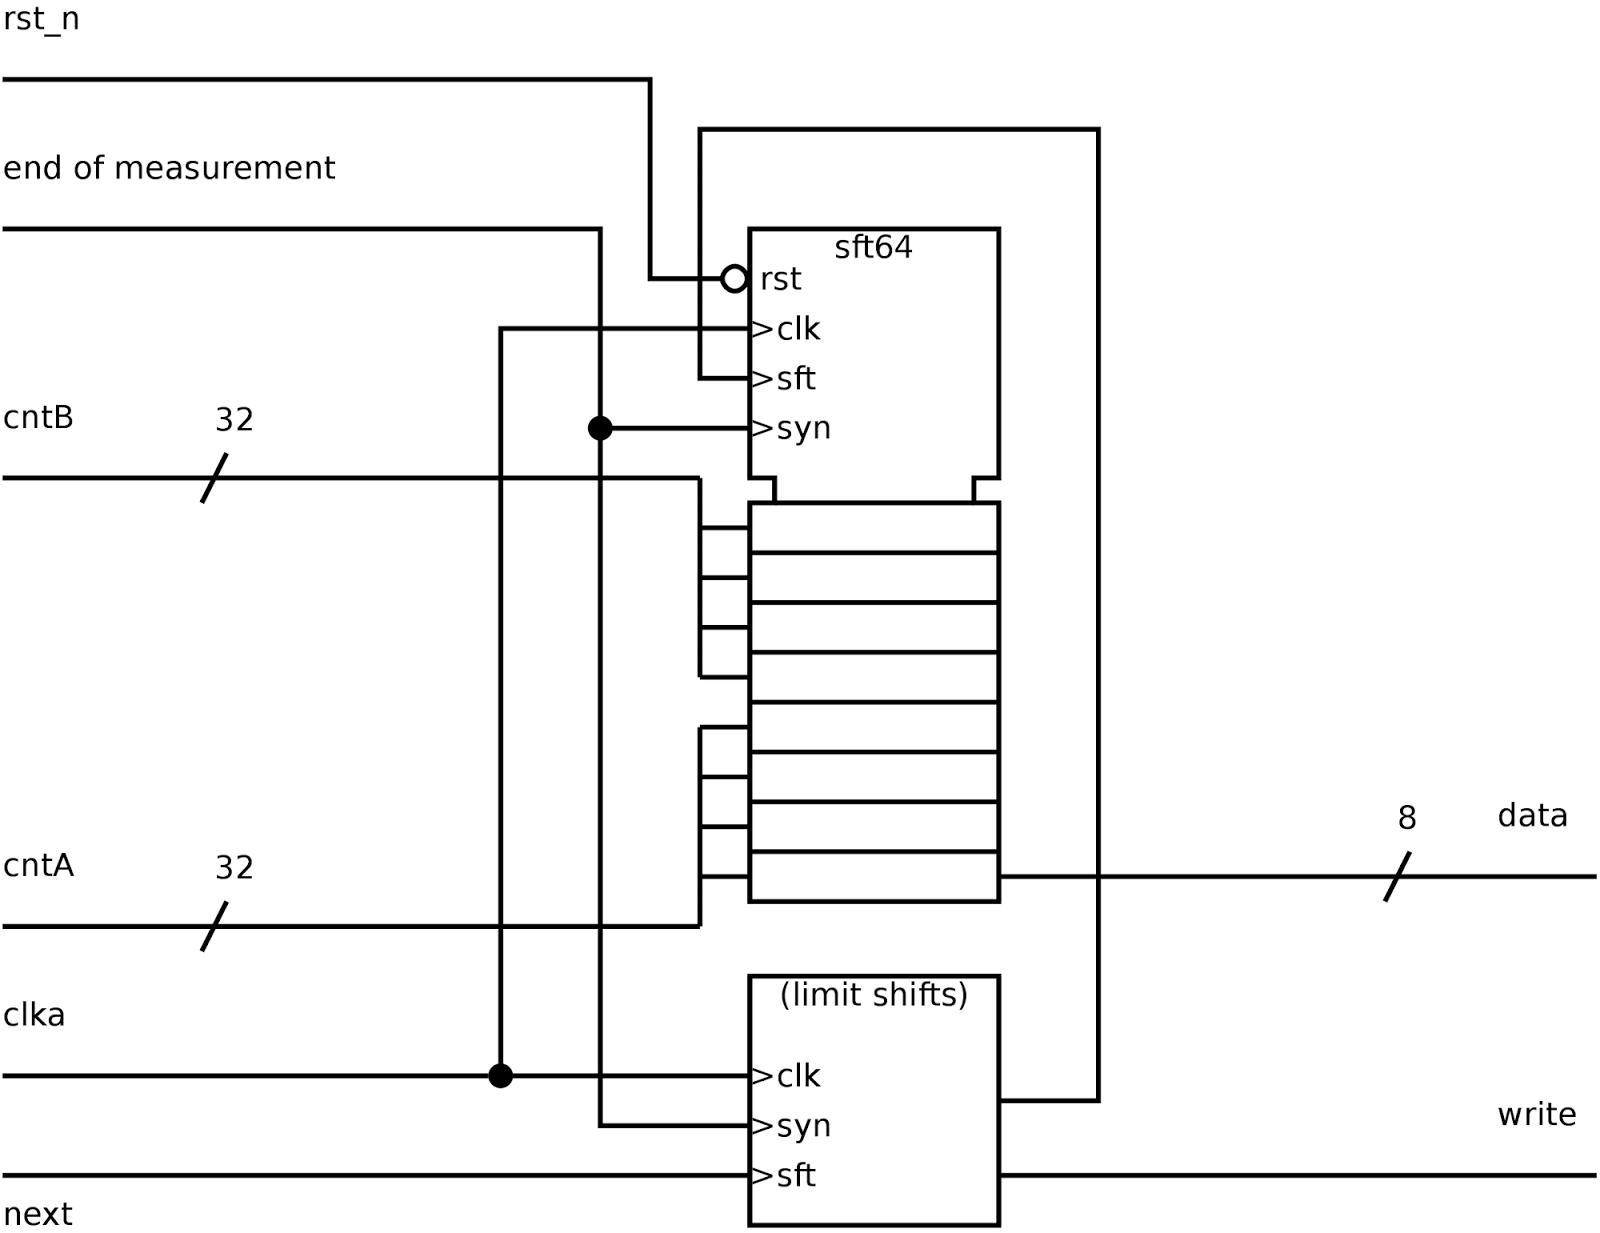
\includegraphics[width=0.75\textwidth]{images/fpga_serialization}
\par\end{centering}

\caption{\label{fig:Serialization-of-two-32-bit-counter-values}Serialization
of two 32-bit counter values}
\end{figure}


The serial transmitter (Figure \ref{fig:Serialization-of-two-32-bit-counter-values})
is only capable of sending one byte at a time, thus a shift register
is needed to serialize the 64 bits into 8 bit chunks.

Each time a new pair of counter values is generated, the values are
loaded into the shift register (\textquotedblleft{}\texttt{syn}\textquotedblright{}
signal) and a \textquotedblleft{}\texttt{write}\textquotedblright{}
pulse is sent to the UART to initiate a transmission. As soon as the
UART is capable of consuming one more byte, the \textquotedblleft{}\texttt{next}\textquotedblright{}
signal is triggered by the UART. This causes a shift to the next byte
and a subsequent \textquotedblleft{}\texttt{write}\textquotedblright{}
pulse until 8 bytes are sent (7 shifts total).


\section{UART}

Based upon \href{http://www.ece.ualberta.ca/~elliott/ee552/studentAppNotes/1999f/UART/txmit.vhd}{http://www.ece.ualberta.ca/$\sim$elliott/ee552/studentAppNotes/1999f/UART/txmit.vhd}
but modified interface behaviour and replaced baud rate generation
with a more flexible clock divider that is not limited to dividers
to the power of two.

The two counter values are sent in little-endian%
\footnote{http://en.wikipedia.org/wiki/Little-endian%
} format as seen in figure \ref{fig:Binary-format-for-counters}.

\begin{figure}[h]
\noindent \begin{centering}
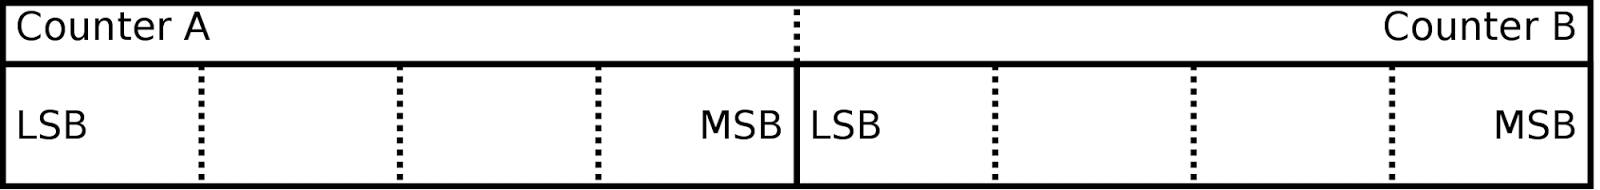
\includegraphics[width=0.8\textwidth]{images/fpga_endianess}
\par\end{centering}

\caption{\label{fig:Binary-format-for-counters}Binary format for counter values}
\end{figure}



\subsubsection*{Example of a transmission and it\textquoteright{}s decoding:}

FPGA sends:
\begin{verse}
\texttt{0xA4 0xF0 0xFA 0x02} for counter A and\texttt{}~\\
\texttt{0xF8 0x96 0x98 0x00} for counter B 
\end{verse}
Server decodes: 
\begin{verse}
50,000,036 (\textasciitilde{}50MHz) for counter A and \\
10,000,120 (\textasciitilde{}10MHz) for counter B
\end{verse}
\pagebreak{}


\section{Detailed Schematic}

\begin{figure}[H]
\noindent \centering{}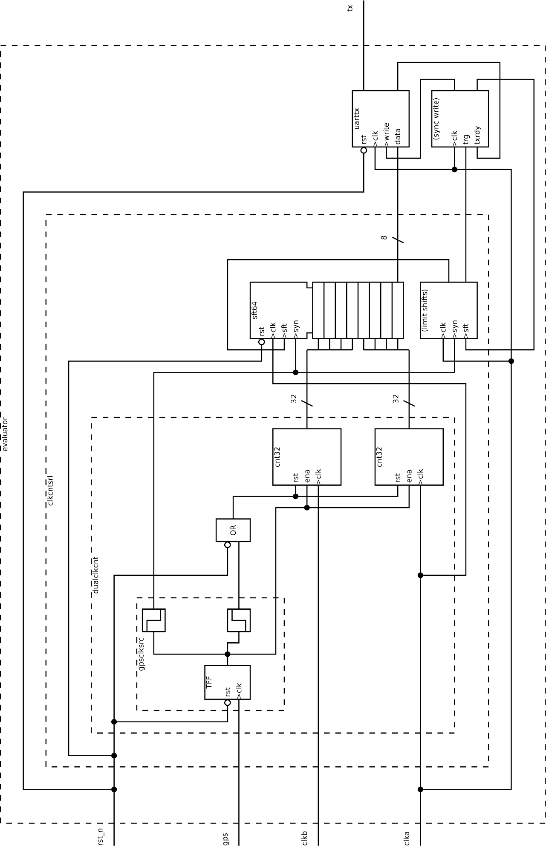
\includegraphics[height=0.9\textheight]{images/fpga_complete}
\end{figure}



\chapter{Server}

The server is programmed using Python%
\footnote{http://en.wikipedia.org/wiki/Python\_(programming\_language)%
}. Python is used because it is a high-level programming language,
which provides a large and comprehensive standard library.

To manage the application environment, the Python package ``virtualenv\textquotedblright{}
is used. With this package it is possible to create a local environment
and only install/activate necessary packages (no root privileges required).
For this application only the Python standard library and two additional
packages are needed:
\begin{description}
\item [{argparse==1.2.1}] (to manage program arguments)
\item [{pyserial==2.6}] (to read data from serial/usb ports)\\

\end{description}
To run the server, an Apache Webserver%
\footnote{http://httpd.apache.org/%
} is required. Also the \texttt{mod\_rewrite} and \texttt{mod\_proxy}
modules must be activated. For security reasons, a rewrite of the
event-stream URL to a relative application URL is applied. This is
achieved by a \texttt{.htaccess} file in the root directory of the
website itself:

\begin{Verbatim}[commandchars=\\\{\}]
\PY{n+nt}{\PYZlt{}IfModule} \PY{l+s}{mod\PYZus{}rewrite.c}\PY{n+nt}{\PYZgt{}}
	\PY{n+nb}{RewriteEngine} \PY{k}{on}
	\PY{n+nb}{RewriteRule} events http://localhost:8001/ [NC,L,P]
\PY{n+nt}{\PYZlt{}/IfModule}\PY{n+nt}{\PYZgt{}}
\end{Verbatim}



\section{Components}

The complete program is split into four threads to provide parallel
processing. All threads have a shared message queue to pass messages
from one thread to another. The main program only sets up all threads
and start them. If the main program is terminated, all threads are
terminated as well.

The server can be started with the following command:\\
\texttt{\textbf{python}}\texttt{ manage.py runserver {[}}\texttt{\emph{-{}-debug}}\texttt{{]}}

The option \textquotedblleft{}\texttt{-{}-debug}\textquotedblright{}
can be used to simulate a connected FPGA- and GPS board. It will generate
random values for the two counters and set a fixed GPS position. The
server can be stopped by pressing \texttt{\textbf{Ctrl+C}} on the
keyboard. This will stop all threads and quit the program.


\subsection{FPGAThread}

This thread is reading eight bytes (four bytes for each counter value)
from the serial port connected to the FPGA in an endless loop. This
byte-array is unpacked (little-endian) into two integer variables.
In the next step, these values are encoded as JSON data and finally
put into the shared message queue (Figure \ref{fig:FPGA-thread-activity}).


\minisec{JSON example:}

\begin{lstlisting}
json-data = {
    "cnt1": "50000120",
    "cnt2": "10000048"
}
\end{lstlisting}



\minisec{Message example:}

\begin{lstlisting}
event: clk\ndata: json-data\n\n
\end{lstlisting}


\begin{figure}[H]
\noindent \begin{centering}
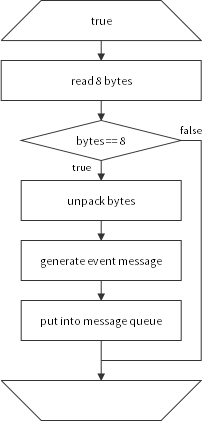
\includegraphics[scale=0.65]{images/server_fpga}
\par\end{centering}

\caption{\label{fig:FPGA-thread-activity}FPGA thread activity diagram}
\end{figure}



\subsection{GPSThread}

This thread (Figure \ref{fig:GPS-thread-activity}) uses an endless
loop to read every byte from the GPS module. Until a new line character
is received, all characters are merged into a sentence. If a sentence
is complete, the required information is parsed from the sentence.
Latitude and longitude must be converted from the degrees/minutes/seconds-format
into the decimal degrees format. After JSON encoding, the data is
also put into the shared message queue.


\minisec{JSON example:}

\begin{lstlisting}
json-data = {
    "time": "17:47:25",
    "date": "18.01.2013",
    "latitude": "...",
    "longitude": "...",
    "altitude": "...",
    ...
}
\end{lstlisting}



\minisec{Message example:}

\begin{lstlisting}
event: gps\ndata: json-data\n\n
\end{lstlisting}


\begin{figure}[H]
\noindent \begin{centering}
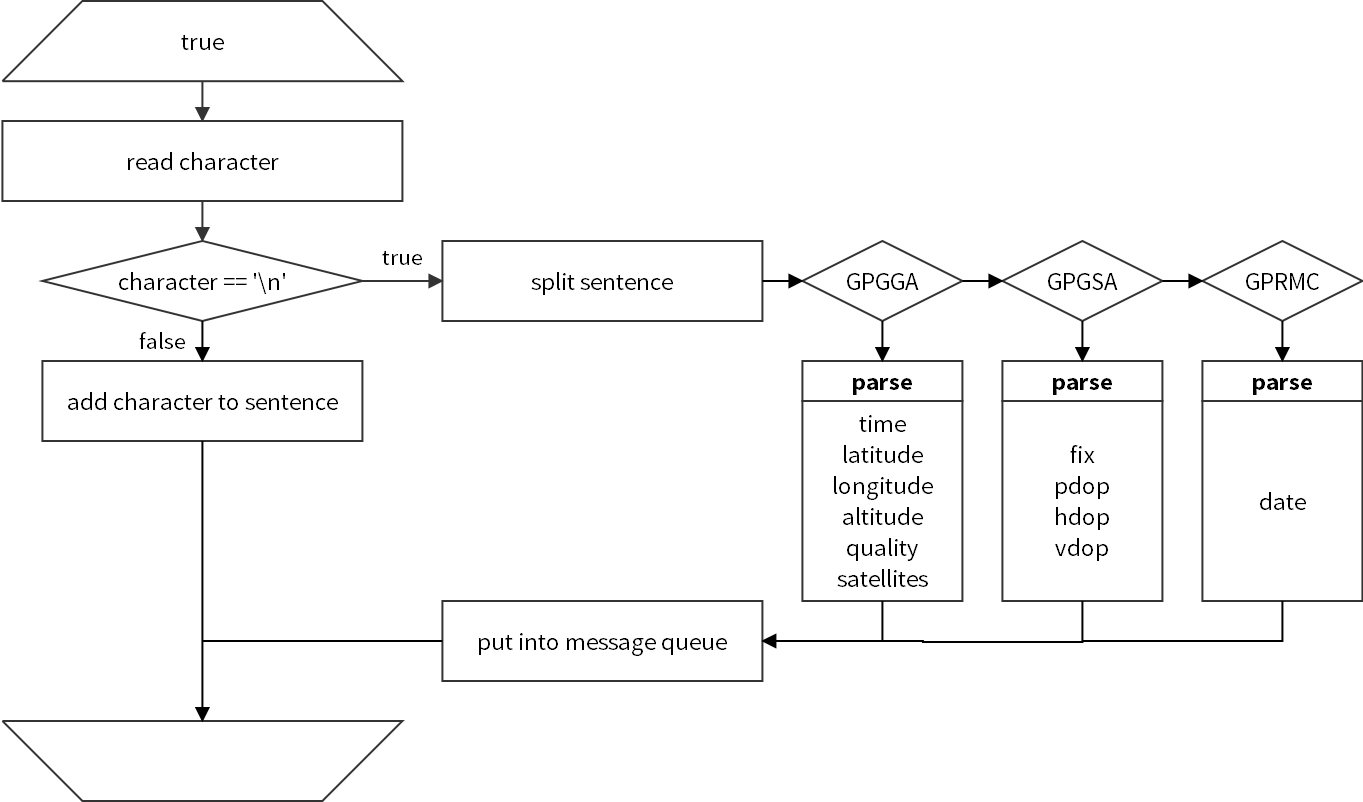
\includegraphics[width=1\textwidth]{images/server_gps}
\par\end{centering}

\caption{\label{fig:GPS-thread-activity}GPS thread activity diagram}
\end{figure}



\subsection{TCPThread}

This thread (Figure \ref{fig:TCP-thread-activity}) is responsible
for the TCP connections to the smartphones. As this is a multithreaded
server, it is possible to connect multiple smartphones simultaneously.
The data is also put into the shared message queue. To close the connection,
the smartphone\textquoteright{}s client has to send a message containing
\textquotedblleft{}\texttt{bye}\textquotedblright{}.


\minisec{JSON example:}

\begin{lstlisting}
json-data = {
    "latitude": "...",
    "longitude": "...",
    "altitude": "...",
}
\end{lstlisting}



\minisec{Message example:}

\begin{lstlisting}
event: ext\ndata: json-data\n\n
\end{lstlisting}


\begin{figure}[H]
\noindent \begin{centering}
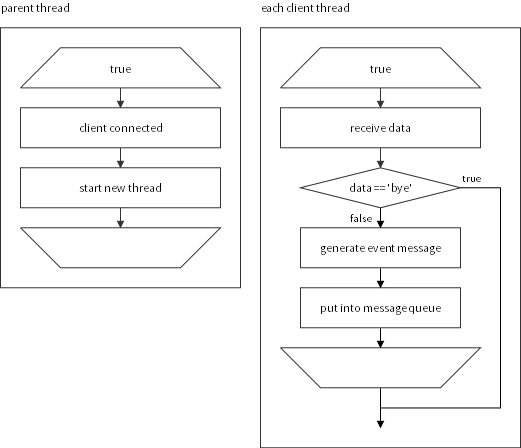
\includegraphics[width=0.75\textwidth]{images/server_tcp}
\par\end{centering}

\caption{\label{fig:TCP-thread-activity}TCP thread activity diagram}
\end{figure}



\subsection{SSEThread}

This thread (Figure \ref{fig:SSE-thread-activity}) is used to transmit
the events from the FPGA-, GPS- and TCP-Thread to the connected web-client.
Basically this thread is a HTTP-Server, whose content-type is changed
to \textquotedblleft{}\texttt{text/event-stream}\textquotedblright{}.
Whenever a new event is available in the shared message queue, it
will be sent to the client.


\minisec{Stream example:}

\begin{lstlisting}
event: type\ndata: data\n\n
\end{lstlisting}


\begin{figure}[H]
\noindent \begin{centering}
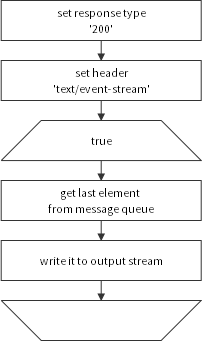
\includegraphics[scale=0.65]{images/server_sse}
\par\end{centering}

\caption{\label{fig:SSE-thread-activity}SSE thread activity diagram}
\end{figure}



\section{Activity Diagram}

\begin{figure}[H]
\noindent \begin{centering}
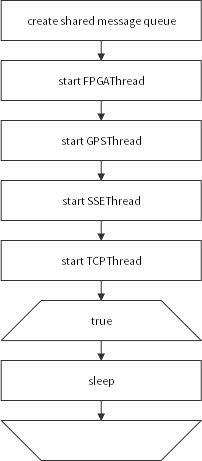
\includegraphics[scale=0.75]{images/server_complete}
\par\end{centering}

\caption{\label{fig:Activity-diagram}Activity diagram}
\end{figure}



\chapter{Client}


\section{Web-Interface}

To display the collected information, a HTML5%
\footnote{http://en.wikipedia.org/wiki/HTML5%
} web-interface has been developed. This web-interface (Figure \ref{fig:User-Interface})
can be opened with every browser%
\footnote{The complete web-interface has been tested with Google Chrome, so
we recommend to use it.%
}. JavaScript%
\footnote{http://en.wikipedia.org/wiki/JavaScript%
} (with jQuery), a client-side scripting language is used to receive
new information from the server and update the interface.

\begin{figure}[h]
\noindent \begin{centering}
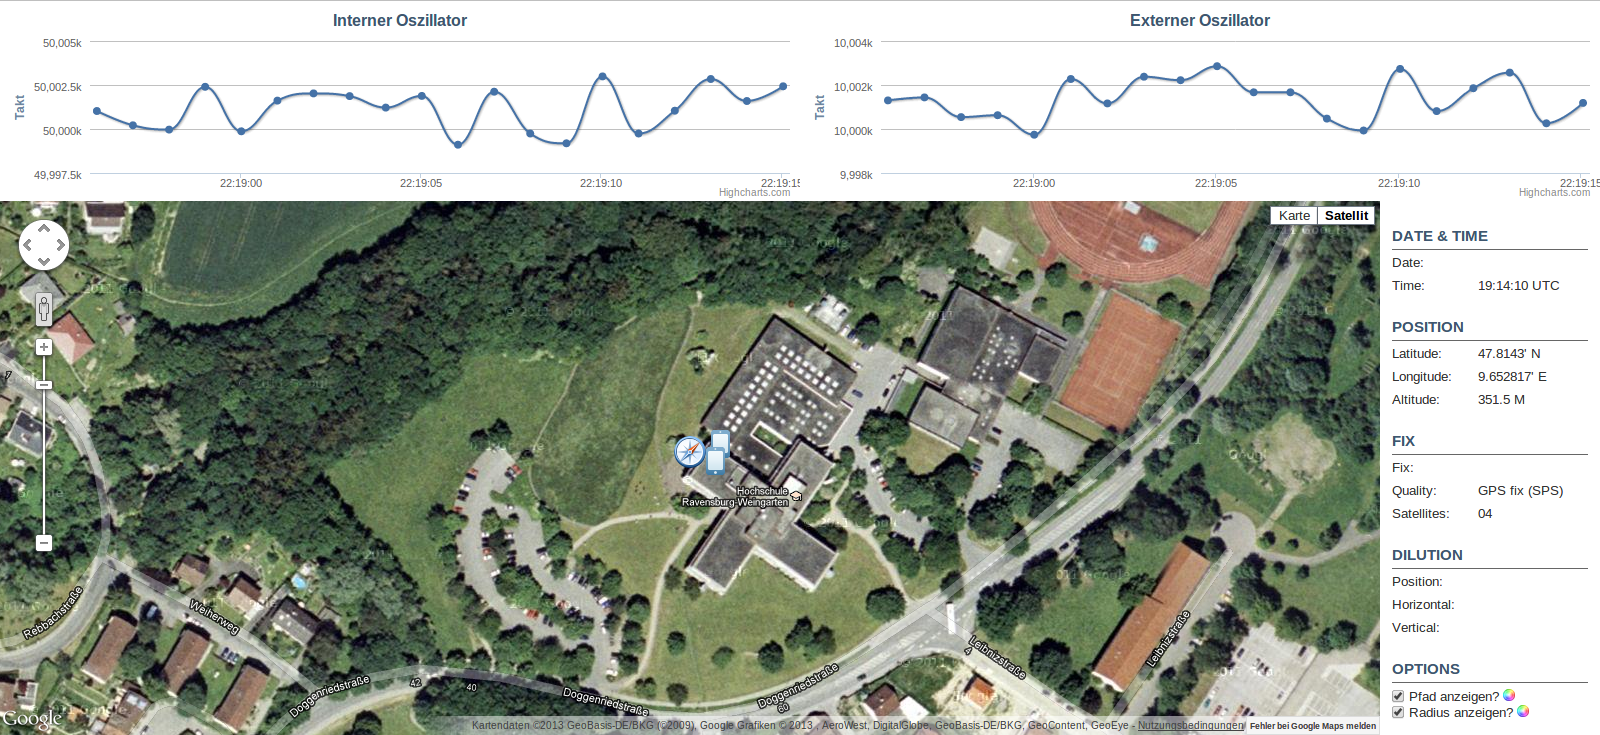
\includegraphics[width=1\textwidth]{images/client_webgui}
\par\end{centering}

\caption{\label{fig:User-Interface}User-Interface}
\end{figure}


The page can be split into three components. The first component is
the map. This map uses the Google Maps JavaScript API%
\footnote{https://developers.google.com/maps/documentation/javascript/?hl=de%
} to display the current position of the GPS board at the center of
the map. In addition, the position of connected Android smartphones
is displayed (see Chapter \ref{sec:Android}). It is also possible
to display the path of the last 100 positions and an estimated precision
(as circle around the icon) of the GPS board.

The second component is the information HUD on the left side. All
important information from the GPS board, like position, fix quality,
number of satellites can be found there. The last component is the
characterization of oscillators. Therefore we used the Highcharts%
\footnote{http://www.highcharts.com/%
} JavaScript library, to display two graphs at the head of the page.
With these graphs the frequency of the oscillators (only the last
20 samples, the value range is adjusted dynamic) is visualized.

The communication with the server is realized via server-send-events%
\footnote{http://en.wikipedia.org/wiki/Server-sent\_events%
} (sse). These events are generated by the SSEThread (see Chapter {[}SSETHREAD{]})
in the server application. On the client side, it is sufficient to
connect to this event-stream and react to the events. The basic functionality
is shown in the next example.


\minisec{Example:}

\begin{lstlisting}[basicstyle={\scriptsize},breaklines=true,language=Java,tabsize=4]
var source = new EventSource('/gps/events'); 
source.addEventListener('clk', function(e) { do something with data }, false); 
source.addEventListener('gps', function(e) { do something with data }, false); 
source.addEventListener('ext', function(e) { do something with data }, false);
\end{lstlisting}


Because the data is encoded as JSON, it is trivial to extract the
required information - JavaScript has a build-in function called \texttt{JSON.parse(e.data)}.
This function parses the JSON data and returns the data as object
or array.


\section{\label{sec:Android}Android}

Since the web-interface already displays the GPS position of the GPS
module, it was obvious that other devices may be shown on the screen,
too.

Android is well suited for this task, as within the Android device
it is possible to retrieve the GPS information of the smartphone itself.
This GPS dataset is transferred to the server, that displays all connected
smartphones. The developed application, is called an Android ``App''
and is shown in the following figures. 

\begin{figure}[h]
\noindent \begin{centering}
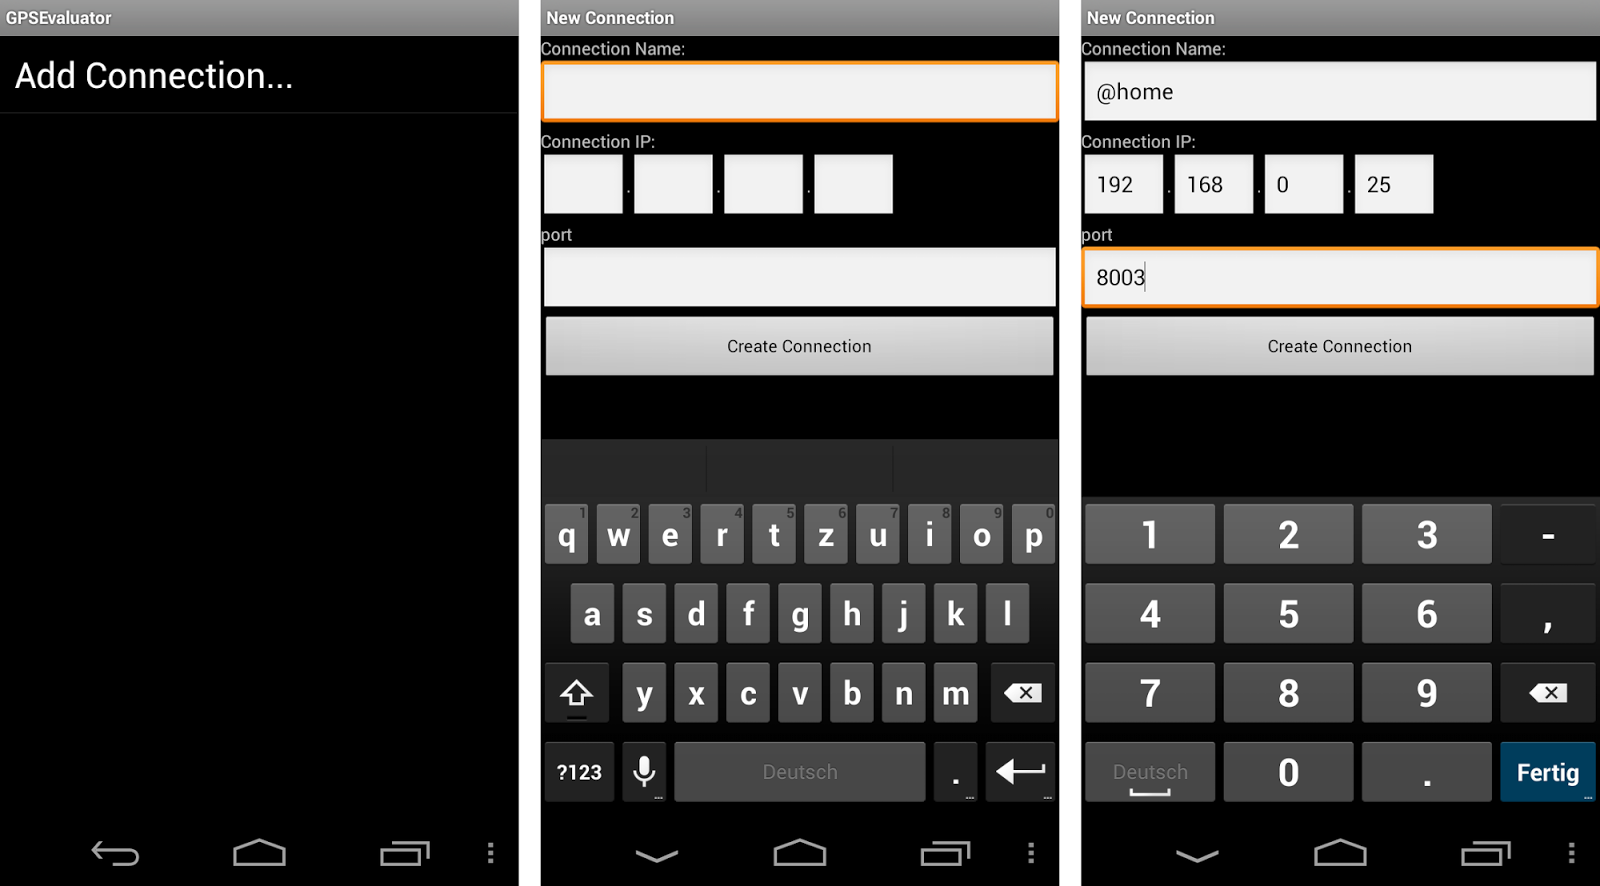
\includegraphics[width=0.95\textwidth]{images/client_add_connection}
\par\end{centering}

\caption{\label{fig:Adding-a-connection}Adding a connection}
\end{figure}


\begin{figure}[h]
\noindent \begin{centering}
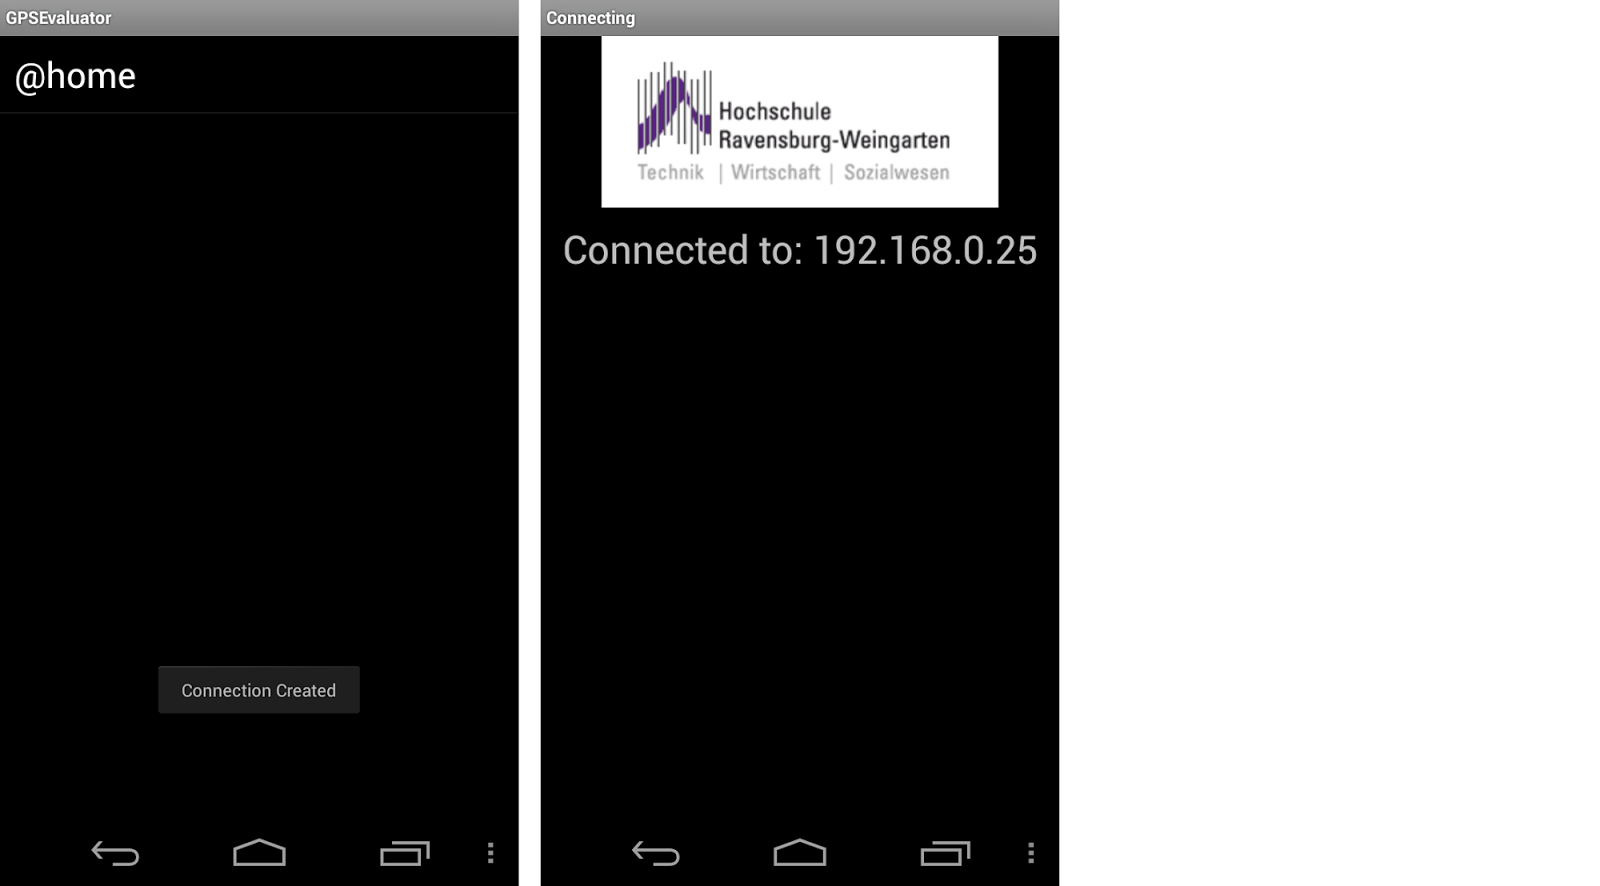
\includegraphics[width=0.95\textwidth]{images/client_connect_server}
\par\end{centering}

\caption{\label{fig:Connect-to-server}Connect to server}
\end{figure}


Figure \ref{fig:Android-activity-diagram} shows the design of the
application.

\begin{figure}[h]
\noindent \begin{centering}
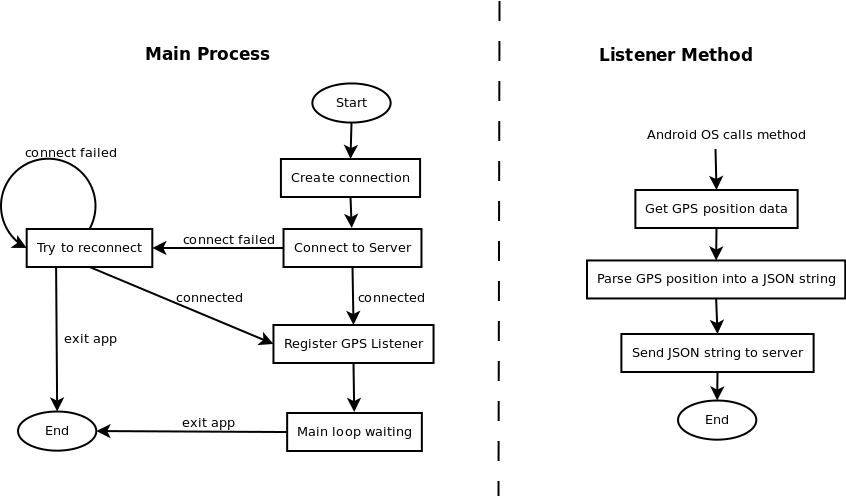
\includegraphics[width=0.9\textwidth]{images/client_design}
\par\end{centering}

\caption{\label{fig:Android-activity-diagram}Android activity diagram}
\end{figure}


The diagram shows that at first, the user has to configure the network
connection to the server by entering it's IP-Address and port. After
this step the connection to the server can be opened. If it is not
possible to establish a connection, the App will repeat the connection
attempt until a connection is established or the user cancels the
connection process. If the connection is established, the App listens
to the GPS data, which is provided by the Android OS. Two parameters
can be chosen that define the update condition of the GPS position: 

A minimum change of the position and additionally a minimum time interval
between two updates can be defined. (current implementation: min.
distance change=1 meter, min. time change=1 second) 

Android calls the method which is responsible for updating the server.
This method shown on the right side of the diagram, is running in
parallel to the main process. The method receives the GPS information
as an argument. This GPS dataset is converted to a JSON string which
contains the Android\textquoteright{}s Device-ID, latitude, longitude
and the altitude. Further, this generated JSON string is transmitted
to the server which shows a symbol for each smartphone on the map.
This task is repeated until the user stops the App. As the server
is multithreaded, it is possible to connect any number of smartphones.
While testing the GPS device it turns out, that occasionally there
is a difference of about 10-20 meters from the real position. So with
three devices (one GPS device and two Android devices e.g.) it is
possible to make a triangle interpolation to minimize the location
error of the single devices. This referencing process can for example
be done at beginning, but it is currently unimplemented.


\chapter{Statistics}

As shown in Chapter \ref{sec:2x32-Bit-Binary-Counter}, a 32-bit counter
for each oscillator is used. As a result no dividers are necessary.
The obtained counter values are 100\% accurate, as every pulse of
the oscillator is counted. 

It seems that the counter values fluctuate about plus minus three.
A possible explanation for these differences could be that the noise
on the GPS clock signal affect the accuracy of the counting period.
Among other things, this effect depends on the cable length between
GPS module and FPGA board.

For more detailed statistics, more sample data as currently available
would be necessary.


\chapter{Problems}

The one-second signal between GPS module and FPGA is prone to noise
and other disturbances caused by long wires. These circumstances manifest
in incorrect counter values.

Unclean rising and/or falling edges produced measurement phases shorter
than one second. The most common error appeared after the falling
edge on the signal: The oscillations after the falling edge resulted
in falsely detected rising-edges that produced counter values amounting
a fifth of the expected values (the one-second signal of the GPS module
has a high-time of a fifth of a second). This effect emerged only
on certain device configurations. 

To mitigate this problem, shorter wires have been used. Additionally
some experimentation was done on where to connect the individual device\textquoteright{}s
power supplies for best signal quality. Following images are taken
from an oscilloscope connected to the GPS clock signal:

\begin{figure}[H]
\noindent \begin{centering}
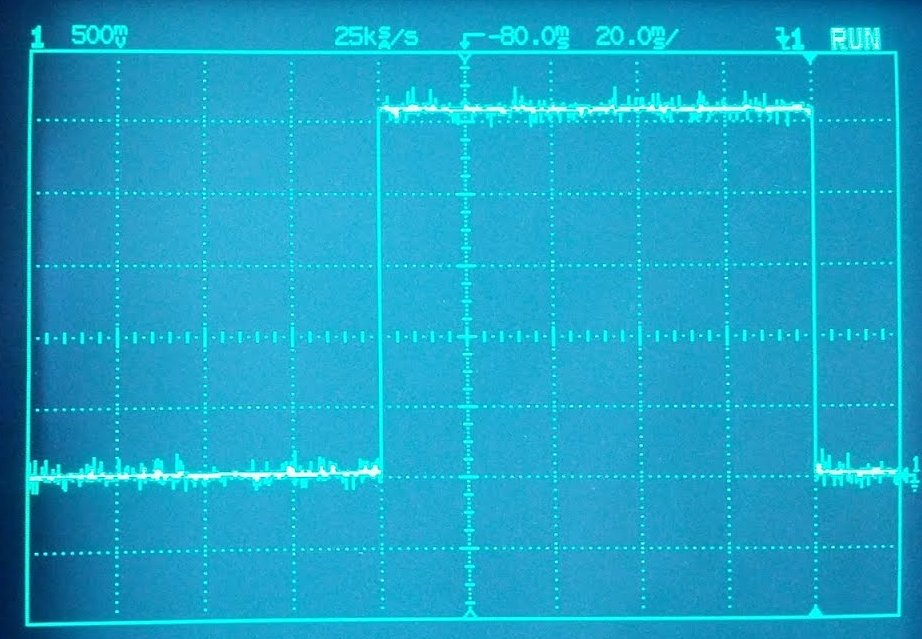
\includegraphics[width=0.5\textwidth]{images/problem_1}
\par\end{centering}

\caption{GPS signal pulse}
\end{figure}


\begin{figure}[H]
\noindent \begin{centering}
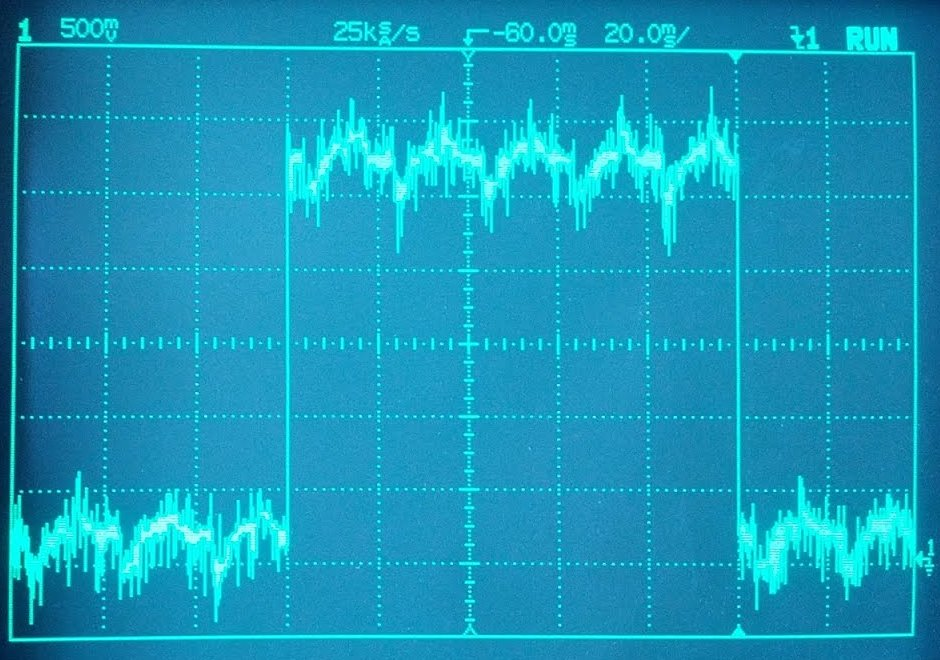
\includegraphics[width=0.5\textwidth]{images/problem_2}
\par\end{centering}

\caption{Noisy GPS signal pulse}
\end{figure}
\begin{figure}[h]
\noindent \begin{centering}
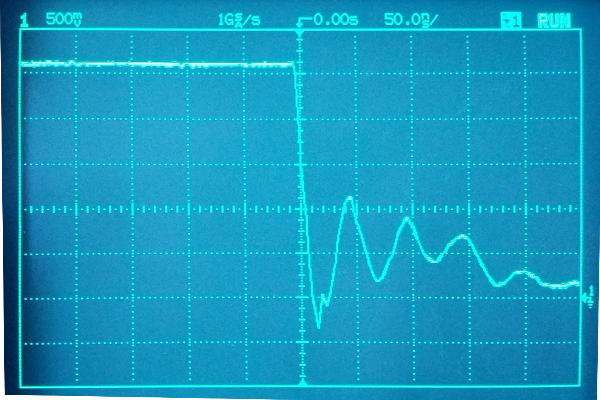
\includegraphics[width=0.5\textwidth]{images/problem_3}
\par\end{centering}

\caption{Falling-edge oscillations}
\end{figure}



\chapter{Summary}

For us as computer scientists this project was a great experience.
Common computer scientists only program the software running on some
hardware. Until this course, nobody of us had experience with designing
and implementing hardware circuits itself using VHDL. At the beginning
we had some problems getting used to the idea of VHDL programming,
as VHDL is a descriptive language that differs from common programming
languages like C, C++ or Java.

It was more effective to learn about hardware-software-co-design working
on a hands-on project than just learning the theoretical approach.
There are many possibilities on how to use GPS information in applications,
so we implemented additional functionality in our project (e. g. display
current position on map, connect Android smartphones). The logic is
realized in VDHL and could successfully be synthesised on our target
system. Both oscillator frequencies are measured correctly and sent
to the server. Also the GPS board and all connected smartphones transfer
their position information to the server. The server forwards all
this information to the client, which in turn displays the data in
a user-friendly manner.

\vfill{}



\lyxaddress{\noindent \begin{center}
\href{https://github.com/wydler/gps-evaluator}{https://github.com/wydler/gps-evaluator}
\par\end{center}}

\pagebreak{}

\bibliographystyle{plain}
\phantomsection\addcontentsline{toc}{chapter}{\bibname}\bibliography{refs}

\end{document}
